\chapter{Use-Case Diagramm}

Im folgenden Kapitel werden die Use-Cases und Akteure der zu implementierenden Anwendung zuerst aufgelistet und anschließend genauer erläutert.
Danach folgen die auf den Use-Cases und Akteuren beruhenden Diagramme.

\section{Vorüberlegung}

\begin{enumerate}[itemsep= -0.25 cm]
    \item Buchung verwalten
    \begin{enumerate}[itemsep= -0.25 cm]
        \item Buchung eines Termins
        \item gebuchten Termin bearbeiten
        \item Stornierung eines Termins
        \item Buchung einsehen
    \end{enumerate}
    \item Kunde verwalten
    \begin{enumerate}[itemsep= -0.25 cm]
        \item neuen Kunden Anlegen
        \item bestehenden Kunden löschen
        \item bestehenden Kunden bearbeiten
        \item bestehenden Kunden einsehen
    \end{enumerate}
    \item Mitarbeiter verwalten
    \begin{enumerate}[itemsep= -0.25 cm]
        \item neuen Mitarbeiter anlegen
        \item bestehenden Mitarbeiter löschen
        \item bestehenden Mitarbeiter einsehen
        \item Mitarbeiterrolle bearbeiten
    \end{enumerate}
    \item Fahrzeug verwalten
    \begin{enumerate}[itemsep= -0.25 cm]
        \item neues Fahrzeug anlegen 
        \item bestehendes Fahrzeug bearbeiten
        \item bestehendes Fahrzeug löschen
        \item bestehendes Fahrzeug einsehen
        \item Wartungstermin festlegen
        \item Fahrzeugbild hochzuladen
        \item Standortveränderung eines Fahrzeugs einplanen
    \end{enumerate}
    \item Rabattaktion verwalten
    \begin{enumerate}[itemsep= -0.25 cm]
        \item neue Rabattaktion anlegen
        \item bestehende Rabattaktion löschen
        \item bestehende Rabattaktion einsehen
    \end{enumerate}
    \item Auswahlliste bearbeiten
    \item Back-Up verwalten
    \begin{enumerate}[itemsep= -0.25 cm]
        \item neues Back-Up erstellen
        \item Daten importieren
        \item Daten exportieren
    \end{enumerate}
    \item Standort verwalten
    \begin{enumerate}[itemsep= -0.25 cm]
        \item neuen Standort anlegen
        \item bestehenden Standort bearbeiten
        \item bestehenden Standort löschen
        \item bestehenden Standort einsehen
    \end{enumerate}
    \item Ausrüstung verwalten
    \begin{enumerate}[itemsep= -0.25 cm]
        \item neuen Ausrüstungsgegenstand anlegen
        \item bestehenden Ausrüstungsgegenstand bearbeiten
        \item bestehenden Ausrüstungsgegenstand löschen
        \item bestehenden Ausrüstungsgegenstand einsehen
    \end{enumerate}
    \item Konfiguration der Benutzeroberfläche ändern
    \item Rechnung verwalten
    \begin{enumerate}[itemsep= -0.25 cm]
        \item neue Rechnung anlegen
        \item bestehende Rechnung archivieren
        \item bestehende Rechnung einsehen
    \end{enumerate}
    \item Mahnung versenden
    \item In System einloggen
\end{enumerate}

\section{Use-Case Analyse}

\textbf{Akteure:}


\begin{itemize}
    \item \textbf{Nutzer}: Der Nutzer ist ein Akteur, der im Rahmen von konzeptionellen Vorüberlegungen entstanden ist. An sich gibt es keinen 'Nutzer' im System, doch beschreibt dieser Akteur die Use-Cases, die sowohl von 'Personalmitarbeiter' als auch von 'Organisator' und 'Administrator' durchgeführt werden.
    \item \textbf{Personalmitarbeiter}: Ein Personalmitarbeiter ist ein Angestellter des Car-Sharing-Unternehmens, welcher sich um die Personal-Verwaltung kümmert. Hauptsächlich arbeitet er mit dem zusätzlichen Verwaltungssystem, doch hat er in der Desktopanwendung die Aufgabe der Verwaltung aller Mitarbeiter und Kundendaten.
    \item \textbf{Organisator}: Organisatoren sind die Mitarbeiter des Unternehmens, die aktiv in der Filiale arbeiten und Kundenkontakt pflegen. Organisatoren bearbeiten alle Anfragen von Kunden in der Filiale und ermöglichen einen ununterbrochenen Geschäftsablauf. 
    \item \textbf{Administrator}: Administratoren
    sind für die technischen Aspekte der Firmenarbeit und das Funktionieren der Systeme zuständig. Sollten Probleme und Fehler auftreten, so ist es die Aufgabe der Administratoren diese Fehler zu beheben. Die Datensicherung fällt auch in diesen Bereich. Weiterhin sollen Administratoren Zugriff auf alle anderen Daten haben und auch die Rollen der Mitarbeiter verwalten.
    \item \textbf{Kunde}: Den Kunden betrifft im Konzept der Desktopanwendung keine systembezogenen Bedeutung. In Zukunft soll der Kunde mithilfe einer Webanwendung seine Termine online vereinbaren können. Diese Webanwendung existiert momentan jedoch noch nicht und deren Implementierung ist auch noch nicht geplant. Daher müssen die Kunden zur Terminvereinbarung in eine Filiale kommen, wo ein Organisator die Buchung in das System einträgt. Da der Organisator ohne die Interaktion mit dem Kunden bestimmte Use-Cases, wie zum Beispiel die Terminvereinbarung, nicht erfüllen kann, wird auch der Kunde in dieser Analyse betrachtet.
    \item \textbf{Werkstatt}: Eine Werkstätte hat keinen direkten Zugriff auf die Anwendung, jedoch wird die Werkstatt, ähnlich wie der Kunde, für den Datenfluss bestimmter Use-Cases benötigt. Daher wird die Werkstatt in dieser Analyse ebenfalls erwähnt.
\end{itemize}


\textbf{Use-Cases:}


Die Car-Sharing-Anwendung, welche im Rahmen des Programmentwurfs erstellt werden soll ist ausschließlich eine Verwaltungssoftware. Ein Großteil der Interaktionsmöglichkeiten mit dem Programm ist das Erstellen und Bearbeiten von verschiedensten Datensätzen. 
In den Tabellen \ref{tbl:usecases1}, \ref{tbl:usecases2} und \ref{tbl:usecases3} von Seite \pageref{tbl:usecases1} bis \pageref{tbl:usecases3} erfolgt zu jedem erstellten Use-Case eine wörtliche Erklärung. Wichtig zu betrachten ist dabei, dass alle aufgeführten Verwaltungsaufgaben mit Ausnahme einiger Fälle auf dem gleichen Konzept basieren: neuen Datensatz erstellen, bestehenden Datensatz bearbeiten, bestehenden Datensatz löschen oder bestehenden Datensatz einsehen.

Die analytische Darstellung der Use-Cases in Diagrammform erfolgt später in zwei Schritten. Der erste Ansatz ist ein  Überblick über die grob definierten Use-Cases. Die erwähnten Use-Cases, die 'verwalten' enthalten sind eine Zusammenfassung aus den Unterfunktionen 'anlegen, bearbeiten, einsehen und löschen'. In einigen Fällen kommen weitere Unter-Use-Cases hinzu. Exemplarisch dafür wird ein zweites Diagramm erstellt, welches diese Aufteilung genauer beschreiben wird. Die Erstellung von allen auftretenden Hierarchiestufen der Use-Case-Diagramme ist im Rahmen des Programmentwurfs nicht zielführend, müsste in einem realen Projekt aber vollständig ausgebaut werden. 

\newpage

\begin{table}[ht]

    \begin{onehalfspace}

    \begin{tabular}{l | p{12.5cm}}
        \hline
        Use-Case 1: & Ein Kunde kann vor Ort in der Filiale einen Termin buchen. Dazu wird der Terminwunsch des Kunden entgegengenommen und der Filialmitarbeiter trägt den Termin als Buchung ins System ein. Zusätzlich ist es nötig, bestehende Buchungen bearbeiten zu können, sollte sich z.B. der Zeitraum der Buchung auf Wunsch des Kunden ändern. Es existiert auch der Fall, dass eine Buchung storniert wird, was bis zu 10h vor dem gebuchten Termin möglich ist. Die Mitarbeiter sollen natürlich auch bestehende Buchungen einsehen können.\\
        \hline
        Use-Case 2 & In Anlehnung an die Erkenntniss, dass alle Verwaltungsaufgaben gleiche Grundaufgaben abdecken müssen, trifft dies auch auf die Verwaltung der Kundendatensätze zu. Ein Unternehmen hat immer einen dynamischen Kundenstamm. Es kommen neue Kunden hinzu, bestehende Kunden benötigen eine Datenanpassung (z.B. bei Änderung von Kontakt- oder Addressinformationen), die Daten müssen für die Mitarbeiter einsehbar sein und auf Kundenwunsch kann der Kunden-Account auch geschlossen werden.\\
        \hline
        Use-Case 3 & Neben den Kunden muss es auch einen Datenstamm mit Mitarbeiterdaten geben. Im Lastenheft wurde hervorgehoben, dass die Datenverwaltung der Mitarbeiter (Gehalt, Zahlungsinformationen, etc.) in einem gesonderten System stattfindet. Bei der Mitarbeiterverwaltung in der Desktopanwendung ist ausschließlich die Verwaltung auf Rollenverteilung vorgesehen. Trotzdem werden dafür die Mitarbeiter auch in diesem System als Datensatz benötigt, aber in einem viel geringeren Umfang als im anderen System.\\
        \hline
    \end{tabular}
    \caption{Use-Cases}
    \label{tbl:usecases1}

    \end{onehalfspace}
\end{table}

\clearpage

\begin{table}[ht]

    \begin{onehalfspace}

    \begin{tabular}{l | p{12.5cm}}
        \hline
        Use-Case 4 & Die 'Vermietung' von Fahrzeugen ist der Kernbestandteil des Business-Konzepts des Car-Sharing-Unternehmens. Aus diesem Grund ist der Umfang der Verwaltung von Fahrzeugen umfangreicher als bei anderen Verwaltungsobjekten. Neben den mittlerweile als Standard-Aufgaben klassifizierten Aufgaben benötigen Fahrzeuge weiterhin Wartungstermine (beispielsweise für Reparaturen oder Reifenwechsel). Die Fahrzeuge sind an Standorten abgestellt. Sollten sich zu viele Fahrzeuge an einem Standort befinden, so müssen die Fahrzeuge wieder auf andere Standorte verteilt werden. Schließlich ist noch vorgesehen, dass jeder Fahrzeug-Datensatz Bilder enthält, die das Fahrzeug zeigen. Auch diese Bilder müssen im System hochgeladen werden. \\
        \hline
        Use-Case 5 & Aus verschiedensten Anlässen sollen Rabattaktionen möglich sein. Diese Rabattaktionen müssen grafisch dargestellt werden. Außerdem müssen alle damit verbundenen Konditionen einsehbar sein. Sollte eine Rabattaktion auslaufen, müssen die damit verbundenen Informationen auch wieder aus dem System entfernt werden.\\
        \hline
        Use-Case 6 & Die Benutzeroberfläche der Anwendung soll laut Lastenheft überall wo es sinnvoll ist auf sogenannte Auswahllisten anstelle von Texteingabefeldern zurückgreifen. Diese Listen sollen ebenfalls einfach editierbar sein, um die Auswahlmöglichkeiten schnell anpassen zu können.\\
        \hline
        Use-Case 7 & Der geforderte Datenimport und -export wurde unter dem Use-Case 'Back-Up verwalten' zusammengefasst. Exportierte Daten sollen entweder direkt als Back-Up verwendet oder für Analyseanwendungen weiterverwendet werden. Der Datenimport bezieht sich hauptsächlich auf das Einspielen von Back-Up Datensätzen.\\
        \hline
    \end{tabular}
    \caption{Use-Cases}
    \label{tbl:usecases2}

    \end{onehalfspace}
\end{table}

\clearpage

\begin{table}[ht]

    \begin{onehalfspace}

    \begin{tabular}{l | p{12.5cm}}
        \hline
        Use-Case 8 & Für die Verwaltung von Standorten sind die vier Grundverwaltungsaufgaben 'anlegen', 'bearbeiten', 'löschen' und 'einsehen' vorgesehen. Auch wenn die Standorte weniger dynamisch sind als andere Datensätze, so ist es doch möglich, dass das Unternehmen neue Fahrzeugstandorte aufbaut oder alte Standorte bei zu wenig Auslastung schließt. \\
        \hline
        Use-Case 9 & Die zu verwaltende Ausrüstung ist fahrzeugbezogen. Da das Car-Sharing Unternehmen einen großen Wert auf Kundenzufriedenheit legt und dafür auch mehr anbieten möchte als andere Car-Sharing Unternehmen gibt es zusätzliche Ausrüstung (z.B. Fahrradträger, Dachbox oder Hundetransportbox) die bei verschiedensten Autos an- und abmontiert werden kann. \\
        \hline
        Use-Case 10 & Eine Anforderung an die Desktopanwendung ist die Konfiguration der Benutzeroberfläche. Schriftgröße, Schriftart und Farbmodus sollen wählbar sein. Die Konfiguration findet anwendungsweit (also auf einzelnen Rechnern mit dieser Anwendung) statt.\\
        \hline
        Use-Case 11 & Nach jeder abgeschlossenen Fahrt eines Kunden soll automatisch eine Rechnung erstellt werden. Da die Rechnung ein rechtsgültiges Dokument sein muss, ist die Bearbeitung des generierten Dokuments nicht möglich und auch das Löschen der Rechnung soll nicht möglich sein. Nach Abzahlung der offenen Rechnung soll nur die Archivierung erfolgen, da die Rechnung für 10 Jahre aufgehoben werden muss.\\ 
        \hline
        Use-Case 12 & Sollte die Zahlung einer ausstehenden Rechnung überfällig sein, soll eine Mahnung zur Zahlung erstellt werden, welche an den Kunden geschickt wird. Die exakten finanziellen Abläufe sind wegen des bereits bestehenden Finanzbuchhaltungssystems für diese Arbeit nicht relevant. \\
        \hline
        Use-Case 13 & Voraussetzung für alle Verwaltungsaufgaben ist eine erfolgreiche Anmeldung am System. Je nach zugewiesener Rolle und der damit verbundenen Rechte dürfen verschiedene Datensätze verwaltet werden oder nicht.\\
        \hline

    \end{tabular}
    \caption{Use-Cases}
    \label{tbl:usecases3}

    \end{onehalfspace}
\end{table}

\clearpage

\section{Use-Case Diagramm}

\begin{figure}[!ht]
    \centering
    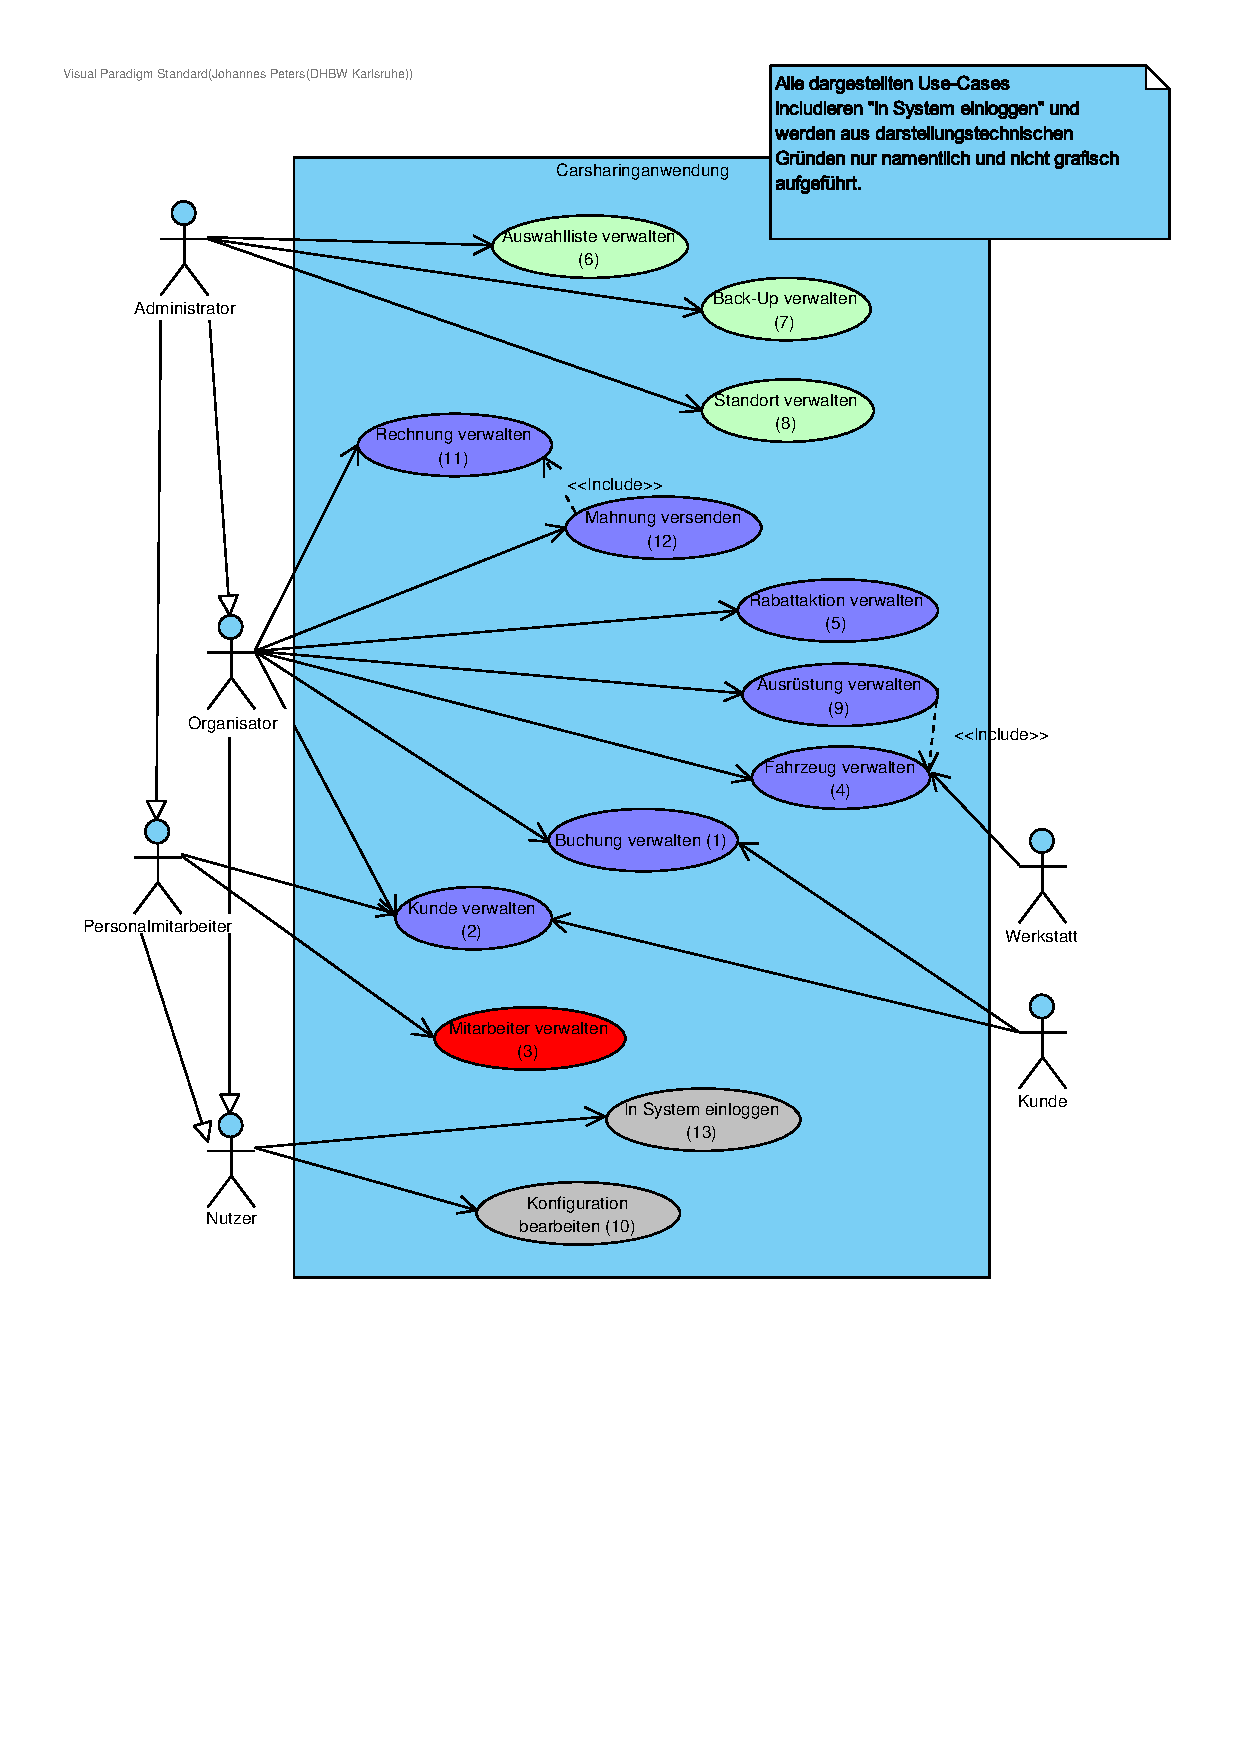
\includegraphics[width=\textwidth, trim = 0cm 8cm 0cm 0cm]{Bilder/Diagramme/Use-Case Diagramm.pdf}
    \caption{Use-Case Diagramm}
    \label{img:use_case_overview}
\end{figure}


\begin{figure}[!ht]
    \centering
    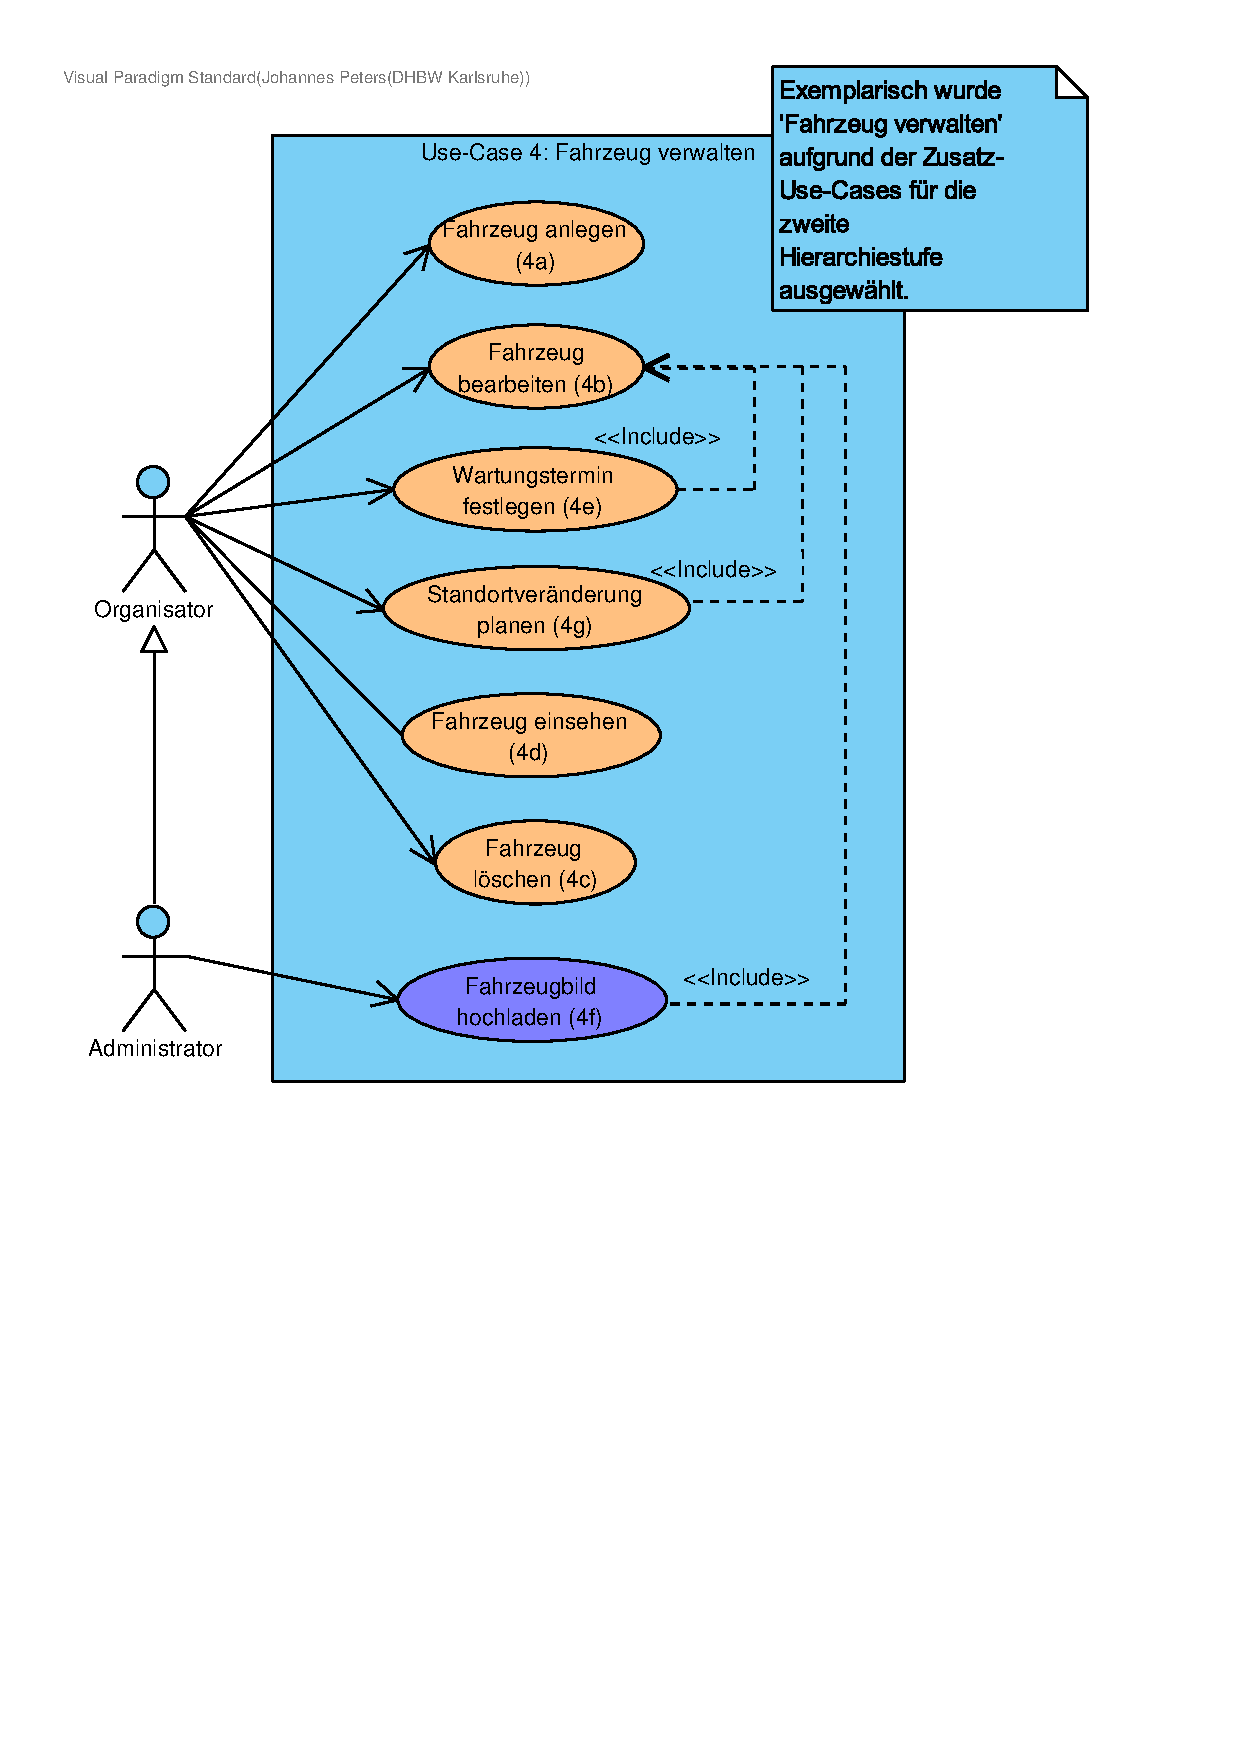
\includegraphics[width=\textwidth, trim = 0cm 11cm 0cm 0cm]{Bilder/Diagramme/Use Case 4_ Fahrzeug verwalten.pdf}
    \caption{Use-Case 4: Fahrzeug verwalten}
    \label{img:use_case_4}
\end{figure}
